\documentclass[journal]{IEEEtran}

% Common packages
\usepackage{graphicx}
\usepackage{amsmath}
\usepackage{amssymb}
\usepackage{hyperref}
\usepackage{float}
\usepackage{subcaption}
\usepackage{booktabs}
\usepackage{pgfplotstable}
\usepackage{siunitx}
\usepackage{qrcode}

\pgfplotsset{compat=1.18}

\begin{document}

% ---------- TITLE & AUTHOR ----------
\title{<Experiment Title>}
\author{<YOUR NAME> \\
Istanbul University, Department of Physics \\
Instructor: <Instructor Name> \\
Experiment Date: <DD.MM.YYYY>, Report Submission Date: <DD.MM.YYYY>\\
Course \& Section Number: PHYSxxx}

\markboth{Physics Laboratory Reports, <Month Year>}{}

\maketitle

% ---------- ABSTRACT ----------
\begin{abstract}
    Briefly summarize the aim of the experiment, the method, and the main numerical results.
\end{abstract}

% ---------- INTRODUCTION ----------
\section{Introduction}
Provide physical background and motivation. Define the phenomenon and why the experiment is important.

% ---------- THEORY ----------
\section{Theory}
Present the key equations and concepts used in the analysis.
For example:
\begin{equation}
    y = f(x; \theta)
\end{equation}
Explain each symbol clearly.

% ---------- EXPERIMENTAL SETUP ----------
\section{Experimental Setup}
List the equipment and describe the setup.

\begin{itemize}
    \item Light source / apparatus
    \item Detectors / meters
    \item Optical / mechanical components
\end{itemize}

\begin{figure}[H]
    \centering
    % Update the path to a real image in your experiment folder
    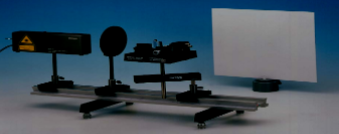
\includegraphics[width=0.8\linewidth]{../IMAGES/setup.png}
    \caption{Schematic diagram of the experimental setup.}
    \label{fig:setup}
\end{figure}

% ---------- PROCEDURE ----------
\section{Experimental Procedure}
Describe step by step how measurements were taken, including ranges, step sizes, and any repetitions.

% ---------- RESULTS ----------
\section{Results}

\subsection{Data Tables}
Insert processed data from CSV files using pgfplotstable, for example:

\begin{table}[H]
    \centering
    \caption{Example data table.}
    \label{tab:data_example}
    \pgfplotstabletypeset[
        col sep=comma,
        string type,
        every head row/.style={before row=\toprule, after row=\midrule},
        every last row/.style={after row=\bottomrule},
        % Adjust column names/styles to your CSV
        columns/col1/.style={column name=$x$},
        columns/col2/.style={column name=$y$}
    ]{../DATA/data.csv}
\end{table}

\subsection{Graphs}
Include plots exported from Python/ROOT:

\begin{figure}[H]
    \centering
    % Update the path to a real plot file
    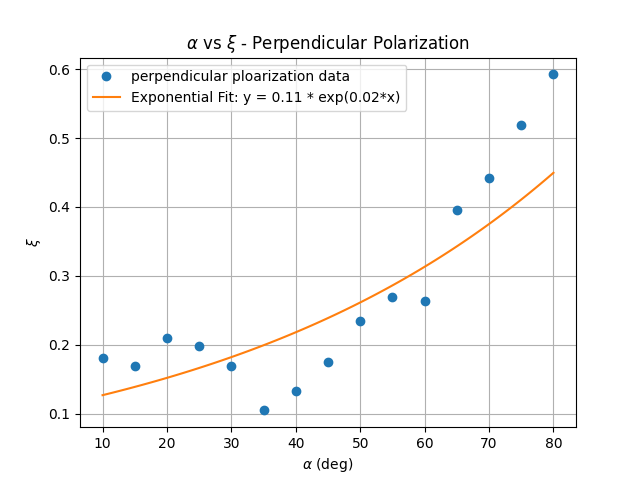
\includegraphics[width=\linewidth]{../plots/plot_example.png}
    \caption{Example plot of measured quantity vs. control variable.}
    \label{fig:plot_example}
\end{figure}

% ---------- DISCUSSION ----------
\section{Discussion}
Interpret the results, compare them with theory, and comment on agreement or discrepancies. Mention estimated parameters and uncertainties.

% ---------- CONCLUSION ----------
\section{Conclusion}
Summarize what was done, main numerical results, and what physical conclusions can be drawn.

% ---------- ADDITIONAL RESOURCES ----------
\section{Additional Resources}
link to GitHub repo or notebook.

\begin{figure}[H]
    \centering
    \begin{minipage}{0.15\textwidth}
        \centering
        \qrcode[height=1.5cm]{https://github.com/<your-user>/<your-repo>}
    \end{minipage}%
    \begin{minipage}{0.2\textwidth}
        \raggedright
        \caption{Access the GitHub repository for source code and related experiments.}
        \label{fig:qr_code}
    \end{minipage}
\end{figure}

\begin{thebibliography}{9}
\bibitem{lab_manual}
    ISTANBUL UNIVERSITY, \textit{[Course] LABORATORY EXPERIMENTS MANUAL}, Department of Physics.

% Add more references as needed

\end{thebibliography}

\end{document}
